% !TeX root = ../main.tex

\chapter{鸡鸭养殖}

...

\section{画图示例}

TIKZ 画线:

\begin{figure}[htb]
  \centering
  % \subcaptionbox{\label{fig:forward-Kinematic-0}}
  %   {
  %     \begin{tikzpicture}[x=1cm, y=1cm, z=0.6cm]
  %       \draw[line width=2mm] (0,0)  -- (0,2);
  %       \draw[red, line width=1.5mm] (0,2)  -- (0,4.12);
  %       \draw[green, line width=1mm] (0,4.12)  -- (0,5.7);
  %       \draw[blue, line width=0.5mm] (0,5.7)  -- (0, 6.4);
  %     \end{tikzpicture}
  %   }
  \subcaptionbox{\label{fig:forward-Kinematic-1}}
    {
      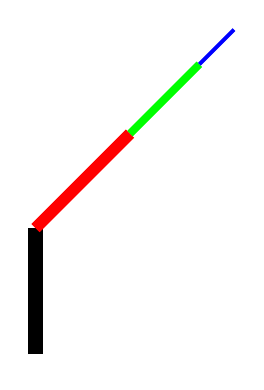
\begin{tikzpicture}[scale=0.8, x=1cm, y=1cm, z=0.6cm]
        \draw[line width=2mm] (0,0)  -- (0,2);
        \draw[red, line width=1.5mm] (0,2)  -- (1.5,3.5);
        \draw[green, line width=1mm] (1.5,3.5)  -- (2.6,4.6);
        \draw[blue, line width=0.5mm] (2.6, 4.6)  -- (3.15, 5.15);
      \end{tikzpicture}
    }
  \subcaptionbox{\label{fig:forward-Kinematics-2}}
    {
      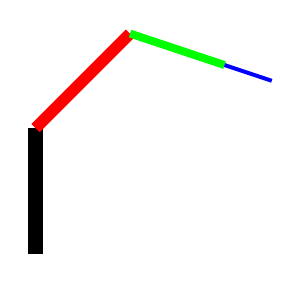
\begin{tikzpicture}[scale=0.8, x=1cm, y=1cm, z=0.6cm]
        \draw[line width=2mm] (0,0)  -- (0,2);
        \draw[red, line width=1.5mm] (0,2)  -- (1.5,3.5);
        \draw[green, line width=1mm] (1.5,3.5)  -- (3,3);
        \draw[blue, line width=0.5mm] (3, 3)  -- (3.75, 2.75);
      \end{tikzpicture}
    }
  \subcaptionbox{\label{fig:forward-Kinematics-3}}
    {
      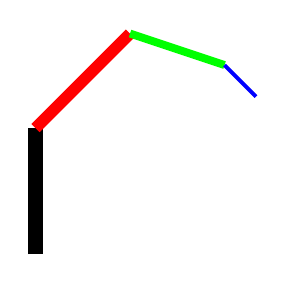
\begin{tikzpicture}[scale=0.8, x=1cm, y=1cm, z=0.6cm]
        \draw[line width=2mm] (0,0)  -- (0,2);
        \draw[red, line width=1.5mm] (0,2)  -- (1.5,3.5);
        \draw[green, line width=1mm] (1.5,3.5)  -- (3,3);
        \draw[blue, line width=0.5mm] (3,3)  -- (3.5,2.5);
      \end{tikzpicture}
    }
  \caption{正向动力学}
  \label{fig:forward-Kinematics}
\end{figure}

JavaScript 代码高亮示例:

\begin{lstlisting}[language=JavaScript]
function setup() { // 初始化骨骼结构
  let current = root;
  for(const bone in bones) { // 遍历骨骼(可能存在多个顺序)
    const next = bone.mesh;  current.child = next;  current = next;
  }
}
function draw { // 更新绘制
  while(next) {
    next.update();  next.show();  next = next.child;
  }
}
class Segment { constructor(point, length, angle) {...}  update() { /* 根据父节点更新位置 */ } }
\end{lstlisting}


\subsection{公式示例}

欧拉角转四元数公式:
\begin{equation}
  \begin{aligned}
  \mathbf{q} &= \mathbf{q}_z \mathbf{q}_x \mathbf{q}_y \\
  &={
      \begin{bmatrix}
        \cos(\frac{y}{2})\\0\\0\\\sin(\frac{y}{2})\\
      \end{bmatrix}
    }{
      \begin{bmatrix}
        \cos(\frac{p}{2})\\\sin(\frac{p}{2})\\0\\0\\
      \end{bmatrix}
    }{
      \begin{bmatrix}
        \cos(\frac{r}{2})\\0\\\sin(\frac{r}{2})\\0\\
      \end{bmatrix}
    }\\
  &={
    \begin{bmatrix}
      \cos(\frac{p}{2})\cos(\frac{r}{2})\cos(\frac{y}{2})-\sin(\frac{p}{2})\sin(\frac{r}{2})\sin(\frac{y}{2})\\
      \cos(\frac{p}{2})\cos(\frac{r}{2})\sin(\frac{y}{2})-\cos(\frac{p}{2})\sin(\frac{r}{2})\sin(\frac{y}{2})\\
      \cos(\frac{p}{2})\cos(\frac{r}{2})\sin(\frac{y}{2})+\cos(\frac{p}{2})\sin(\frac{r}{2})\sin(\frac{y}{2})\\
      \cos(\frac{p}{2})\cos(\frac{r}{2})\sin(\frac{y}{2})+\cos(\frac{p}{2})\sin(\frac{r}{2})\sin(\frac{y}{2})\\
    \end{bmatrix}}\\
  \end{aligned}
\end{equation}

四元数转欧拉角时,设 $\mathbf {q} ={\begin{bmatrix}q_{0}&q_{1}&q_{2}&q_{3}\end{bmatrix}}^{T}={\begin{bmatrix}q_{w}&q_{x}&q_{y}&q_{z}\end{bmatrix}}^{T}$,
而求解欧拉角时计算机中的 $arctan$ 与 $arcsin$ 只能获得区间 $(-\frac{\pi}{2},\frac{\pi}{2})$ 的结果,因此使用 $asin$ 替换 $arcsin$,$atan2$ 替换 $arctan$ 函数\cite{babylonZXY},
则:

\begin{equation}
\begin{aligned}
  \begin{bmatrix}
    pitch \\ roll \\ yaw 
  \end{bmatrix}}={
    \begin{bmatrix}
      {\mbox{asin}}(-2(q_z q_y - q_x q_w))\\
      {\mbox{atan2}}(2(q_z q_x + q_y q_w), q_z^2 - q_x^2 - q_y^2 + q_w^2)\\
      {\mbox{atan2}}(2(q_x q_y + q_z q_w), -q_z^2 - q_x^2 + q_y^2 + q_w^2)
    \end{bmatrix}
\end{aligned}
\end{equation}

\subsubsection{插值公式}

\begin{equation}
  y=y_{0}+(x-x_{0}){\frac {y_{1}-y_{0}}{x_{1}-x_{0}}}={\frac {y_{0}(x_{1}-x)+y_{1}(x-x_{0})}{x_{1}-x_{0}}}
\end{equation}


\section{养殖算法}

\subsection{为什么呢}

画立方体:

% draw cube
% https://tex.stackexchange.com/questions/29877/need-help-creating-a-3d-cube-from-a-2d-set-of-nodes-in-tikz
\begin{figure}
  \centering
  \subcaptionbox{切分立方体\label{fig:octree-cube}}
    {
      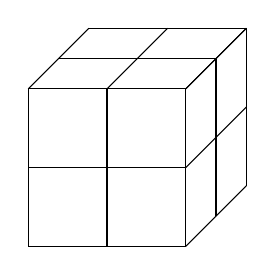
\begin{tikzpicture}
        \foreach \x in{0,...,2}
        {   \draw (0,\x ,2) -- (2,\x ,2);
            \draw (\x ,0,2) -- (\x ,2,2);
            \draw (2,\x ,2) -- (2,\x ,0);
            \draw (\x ,2,2) -- (\x ,2,0);
            \draw (2,0,\x ) -- (2,2,\x );
            \draw (0,2,\x ) -- (2,2,\x );
        }
      \end{tikzpicture}
    }
  \subcaptionbox{对应八叉树\label{fig:octree-tree}}
    {
      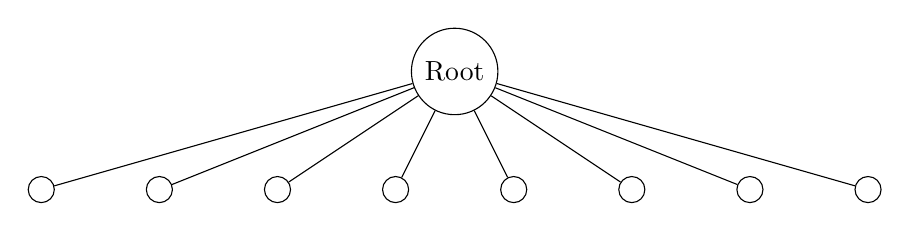
\begin{tikzpicture}
        \tikzstyle{node_style} = [circle,draw=black]
        \node[node_style] {Root}
        child {node[node_style] {}}
        child {node[node_style] {}}
        child {node[node_style] {}}
        child {node[node_style] {}}
        child {node[node_style] {}}
        child {node[node_style] {}}
        child {node[node_style] {}}
        child {node[node_style] {}}
        ;
      \end{tikzpicture}
    }
  \caption{八叉树示例}
  \label{fig:octree}
\end{figure}

放一些看起来高大上的公式。

K-Means 的主要思想是将已知观测集 $(x_1,x_2,...,x_n)$ 划分到 $k$ 个集合($k<=n$),并使每个集合内平方和最小。
即寻找使得下式\eqref{eq:kmeans}最小的聚类 $S_i$($\mu_i$ 是 $S_i$ 中所有点的均值)。
\begin{equation}
  \arg \min_{S_i} \sum_{i=1}^{k} \sum_{x_i \in S_i} (x_i - \mu_i)^2
  \label{eq:kmeans}
\end{equation}

算法实现可主要分为以下两步:分配与更新。

譬如设定存在 $k$ 个初始均值点为 $m_1$,...,$m_k$。

分配:将每个点分配到聚类中,使得集合中的平方和(WCSS)(即平方后的欧式距离)最小。即满足公式\eqref{eq:kmeans_assign}:
\begin{equation}
  S_{i}^{{(t)}}=\left\{x_{p}:\left\|x_{p}-m_{i}^{{(t)}}\right\|^{2}\leq \left\|x_{p}-m_{j}^{{(t)}}\right\|^{2}\forall j,1\leq j\leq k\right\}
  \label{eq:kmeans_assign}
\end{equation}


更新:对于前一步骤得到的每一聚类,重新计算聚类中心(如公式\eqref{eq:kmeans_update}),作为新的均值点。
\begin{equation}
  m_{i}^{{(t+1)}}={\frac  {1}{\left|S_{i}^{{(t)}}\right|}}\sum _{{x_{j}\in S_{i}^{{(t)}}}}x_{j}
  \label{eq:kmeans_update}
\end{equation}


C 代码格式示例:

\begin{lstlisting}[language=c]
  register short *to, *from;
  register count;
  {
    register n = count % 8;
    while (n-- > 0) { 
      *to = *from++;
    }
    n = count / 8;
    if (n == 0) return;     
    do {
      *to = *from++; *to = *from++; *to = *from++; *to = *from++;
      *to = *from++; *to = *from++; *to = *from++; *to = *from++;
    } while (--n > 0)
  }
\end{lstlisting}

三线表:

\begin{table}[h]
  \centering
  \caption{JsPerf (Chrome 84)中循环性能对比}
  \begin{tabular}{p{5cm}p{2cm}}
      \toprule
      \textbf{方法}  & \textbf{Opts/sec} \\
      \midrule
      普通循环 & 165,877  \\
      Duff's Device & 396,801\\
      \bottomrule
  \end{tabular}
  \label{tab:jsperf-efficiency}
\end{table}

\subsubsection{示例图片}

...

多图并列:

\begin{figure}[htbp]
  \centering
  \begin{subfigure}[t]{0.3\textwidth}
  \centering
  
\includegraphics[width=.72\textwidth]{yun-kmeans-3.png}
  \caption{K=3}
  \end{subfigure}
  \begin{subfigure}[t]{0.3\textwidth}
  \centering
  
\includegraphics[width=.72\textwidth]{yun-kmeans-6.png}
  \caption{K=6}
  \end{subfigure}
  \begin{subfigure}[t]{0.3\textwidth}
  \centering
  
\includegraphics[width=.72\textwidth]{yun-kmeans-9.png}
  \caption{K=9}
  \end{subfigure}
  \caption{小云立绘}
  \label{fig:kmeans-png}
\end{figure}


\verb!\href{https://yunyoujun.cn/}{云游君的小站}! 可生成链接\href{https://yunyoujun.cn/}{云游君的小站}。



\section{本章小结}

本章主要介绍...
